\documentclass{article}
\usepackage{graphicx} % Required for inserting images
\usepackage{amsmath}
\usepackage{bm}
\usepackage{amsfonts}

\title{25.02.18 Improving MSP.B}
\author{Xun Zhang \quad \quad Wuyun Siqin \quad \quad Bingsheng Zhang \\ 
Zhejiang University, CHN \\
22221024@zju.edu.cn \quad 3210101763@zju.edu.cn \quad bingsheng@zju.edu.cn}
\date{February 18 2025}

\begin{document}

\maketitle

\section{MSP.B in Mithril}

First of all, we found a new way(actually a new function) to implement the $\mathsf{MSP.B}$ relations in Mithril.
The $\mathsf{MSP.B}$ is as following:

\begin{itemize}
    \item $ivk = \mathsf{MSP.BKey}(\textbf{mvk}, \bm{e_\sigma})$ : Takes a vector $\textbf{mvk}$ of (previously checked) verification keys and weighting seed $\bm{e_\sigma}$, and returns an intermediate aggregate public key.
    \item $(\mu,e_{\bm{\sigma}}) = \mathsf{MSP.BSig}(\bm{\sigma})$: Takes as input a vector of signatures $\bm{\sigma}$ and returns $(\mu,e_{\bm{\sigma}})$ where
$\mu \leftarrow \prod \sigma_i^{e_i}$, where $e_i \leftarrow \textrm{H}_{\lambda}(i,e_\sigma)$ and $e_\sigma \leftarrow \textrm{H}_{p}(\mathbb{\sigma})$.
\end{itemize}

And we also verify the $\mathsf{MSP.B}$ multisignature $\mu$ using aggregated verification key $ivk$ in the circuit.

\section{Original Implementation and Benchmark Results}

For the original implementation of $\mathsf{MSP.B}$, we use a "scalar\_mult" function to aggregate the individual signatures
and pubilc keys. The aggregation relations is as following:

\vspace{0.3cm}


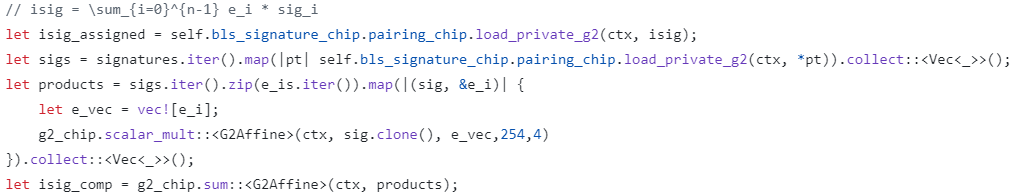
\includegraphics[width=0.9\linewidth]{msp_bkey_isig_code.png}
\\
\\
\\
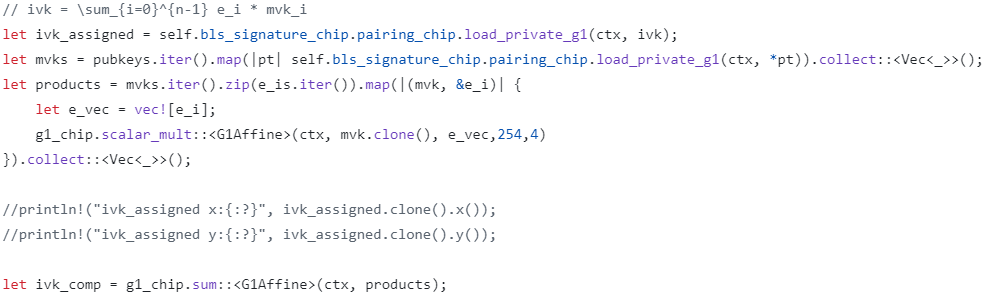
\includegraphics[width=0.9\linewidth]{msp_bkey_ivk_code.png}

\vspace{0.3cm}

We can swap the group if needed. And the "scalar\_mult" function is like:

\vspace{0.3cm}
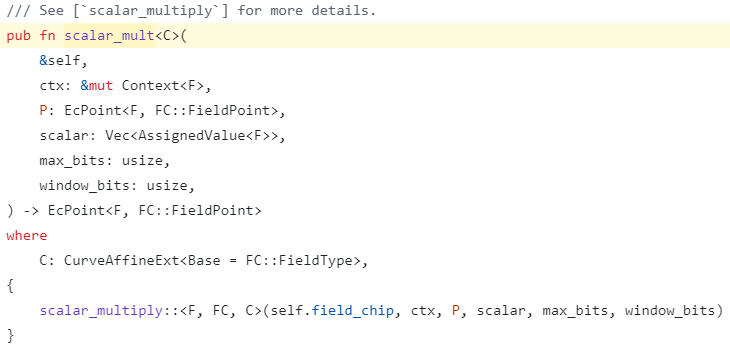
\includegraphics[width=0.9\linewidth]{scalar_mult_code.png}
\vspace{0.3cm}

However, this function is not so efficient, because we need to do a MSM(multi-scalar-multiplication) to every group element. And finally compute the sum of all group elements. But in the relations, one group element is only multiplied by one scalar. 

So "e\_vec" vector in the code only include one scalar variable, and we need to do $n$ times MSM in the circuit to Both $\mathbb{G}_1$ and  $\mathbb{G}_2$ element. This approach caused significant proving cost.


Below is our former benchmark results:

\vspace{0.5cm}
\textbf{Note:} The configuration with Degree , Advice , Lookup Bits , Limb Bits , Num Limbs is 19, 6, 18, 90, and 3, respectively.

\begin{tabular}{c|c|c}
\hline
 \text{num\_aggregation} & \text{proving\_time} & \text{verification\_time} \\
\hline
 4   & 70.5080s  & 14.4204ms  \\ \hline
 8   & 100.3936s & 17.5523ms  \\ \hline
 16  & 145.7191s  & 18.6467ms  \\ \hline
 32  & 251.0654s & 21.7318ms  \\ \hline
 64 & 471.5117s & 30.2121ms  \\ \hline
\end{tabular}\\

When attempting to sign with 128 public keys, the server's 126 GB of RAM and 8 GB swap partition become full, leading to the program being killed. 


\section{Improved MSP.B Implementation}

We conducted a comprehensive inspection of the “halo2-lib" library in response to the previous issues. And we choose a new (implemented) function "variable\_base\_msm\_custom" to complete our aggregation phase. The core code is as following:

\vspace{0.3cm}
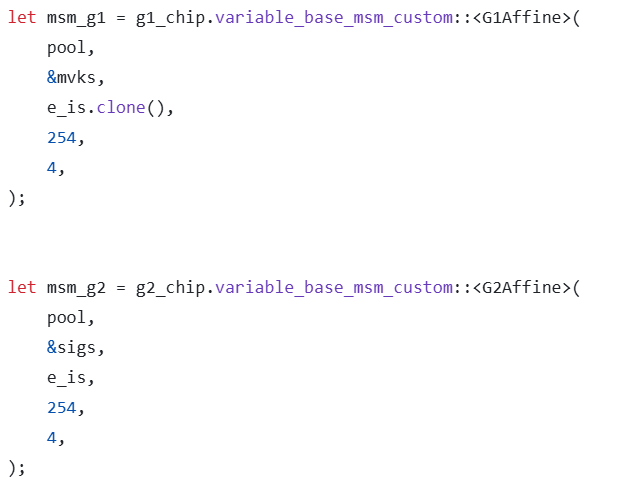
\includegraphics[width=0.9\linewidth]{msp_msm_code.png}
\vspace{0.3cm}

Where "e\_is" is a Vec<Vec<>> type consisting of all aggregation parameters. At first glance, this implementation seems to be the same as the previous one. However, this function is a standard MSM implementation, we don't need to sum the scalar multiplication results manually. See the function details below:


\vspace{0.3cm}
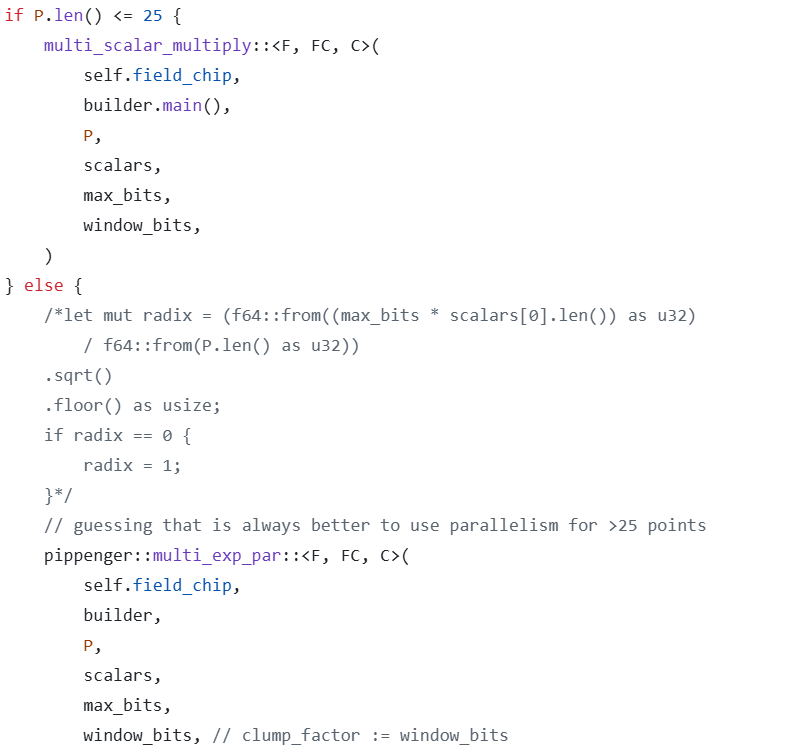
\includegraphics[width=0.9\linewidth]{variable_base_msm_custom.png}
\vspace{0.3cm}

When the length of MSM is bigger than 25, it use a pippenger algorithm to accelerate the MSM.



\section{New Benchmark}

The improved $\mathsf{MSP.B}$ benchmark result is as following:


\vspace{0.5cm}

\begin{tabular}{c|c|c}
\hline
 \text{num\_aggregation} & \text{proving\_time} & \text{verification\_time} \\
\hline
8   & 44.01s  & 14.84ms  \\ \hline
16   & 58.69s & 9.57ms  \\ \hline
 32  & 80.52s  & 10.23ms  \\ \hline
 64  & 125.82s & 15.56ms  \\ \hline
 128 & 217.63s & 18.24ms  \\ \hline
  256 & 422.99s &27.62ms  \\ \hline
\end{tabular}\\

\vspace{0.3cm}
We achieved a $4 \times$ speed-up in this relation. And the parameters are totally same as previous implementation.

\end{document}
